\documentclass{article}

\usepackage{graphicx}
\usepackage{tikz}
\usepackage{tikzsymbols}
\usetikzlibrary{calc,patterns,shapes.geometric}
\pagestyle{empty}
\usepackage[margin=0pt]{geometry}
\geometry{papersize={14in,12in}}

\def\centerarc[#1](#2)(#3:#4:#5){\draw[#1] ($(#2)+({#5*cos(#3)},{#5*sin(#3)})$) arc (#3:#4:#5);}

\begin{document}
	\begin{figure}
		\centering
		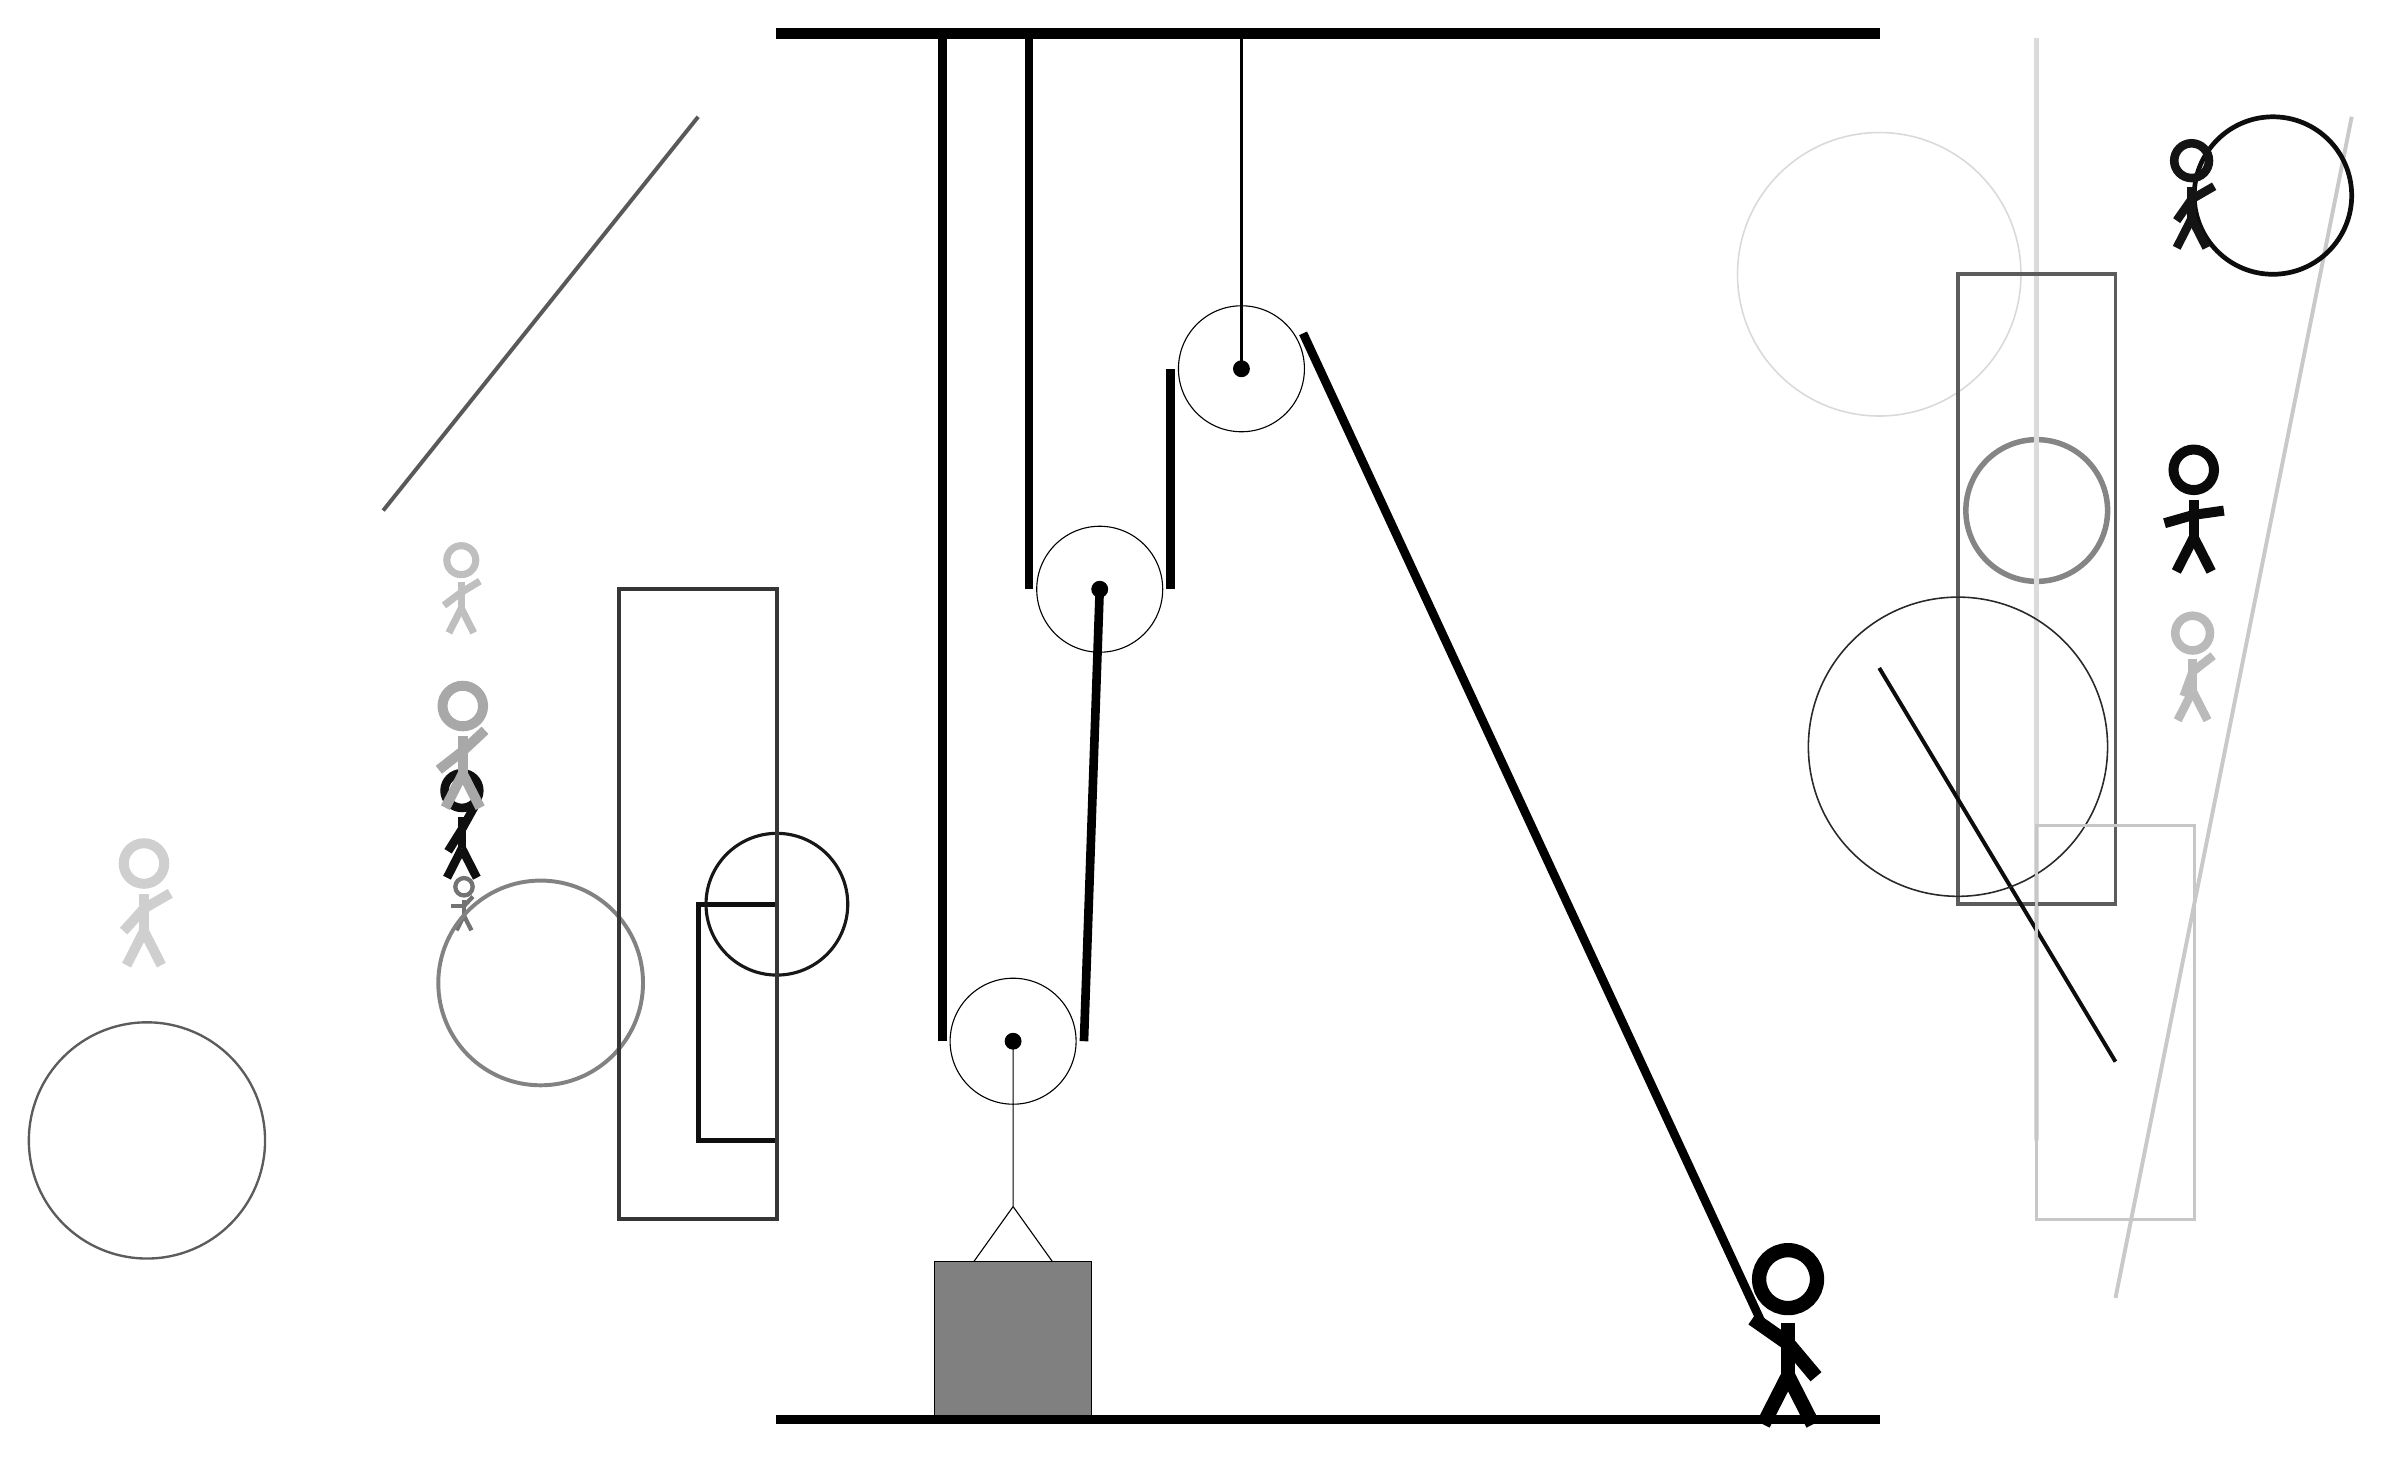
\begin{tikzpicture}
			%%%%% START %%%%%
			
			\draw[fill=black] (-2, 14) rectangle (12, 14.125);
			
			\draw (1, 1.26) circle (0.8);
			\draw[fill=black] (1, 1.26) circle (0.1);
			
			\draw (2.1, 7.0) circle (0.8);
			\draw[fill=black] (2.1, 7.0) circle (0.1);
			
			\node[line width=0.5mm, color=black!55] at (-6, 3) {\Strichmaxerl[3][0][47]};
			
			\draw[line width=0.6mm, color=black!94] (-2, 3) rectangle (-3, 0);
			\draw [line width=0.4mm, color=black!91](-2, 3) circle (0.9);
			\draw[line width=0.5mm, color=black!21](15, -2) -- (18, 13);
			\node[line width=0.3mm, color=black!96] at (16, 8) {\Strichmaxerl[7][16][8]};
			
			\draw [line width=0.2mm, color=black!15](12, 11) circle (1.8);
			
			\draw [line width=0.7mm, color=black!48](14, 8) circle (0.9);
			\node[line width=0.4mm, color=black!27] at (16, 6) {\Strichmaxerl[6][70][38]};
			\draw [line width=0.6mm, color=black!95](17, 12) circle (1.0);
			\draw[line width=0.6mm, color=black!14] (14, 0) rectangle (14, 14);
			\draw[line width=0.5mm, color=black!64] (13, 11) rectangle (15, 3);
			\draw[line width=0.5mm, color=black!95](15, 1) -- (12, 6);
			\node[line width=0.5mm, color=black!94] at (-6, 4) {\Strichmaxerl[6][58][61]};
			\draw [line width=0.2mm, color=black!84](13, 5) circle (1.9);
			\node[line width=0.7mm, color=black!34] at (-6, 5) {\Strichmaxerl[7][38][43]};
			\node[line width=0.7mm, color=black!25] at (-6, 7) {\Strichmaxerl[5][37][31]};
			\node[line width=0.6mm, color=black!19] at (-10, 3) {\Strichmaxerl[7][48][30]};
			\draw [line width=0.3mm, color=black!64](-10, 0) circle (1.5);
			\draw [line width=0.5mm, color=black!49](-5, 2) circle (1.3);
			\draw[line width=0.5mm, color=black!79] (-4, 7) rectangle (-2, -1);
			\draw[line width=0.5mm, color=black!65](-3, 13) -- (-7, 8);
			\node[line width=0.2mm, color=black!92] at (16, 12) {\Strichmaxerl[6][55][30]};
			\draw[line width=0.4mm, color=black!22] (14, -1) rectangle (16, 4);
			
			\draw (3.9, 9.8) circle (0.8);
			\draw[fill=black] (3.9, 9.8) circle (0.1);
			\draw[thick] (3.9, 9.8) -- (3.9, 14);
			
			\draw (1, 1.26) -- (1, -0.84) -- (0.5, -1.54) -- (1.5, -1.54) -- (1, -0.84);
			\draw[fill=black!50] (0, -1.54) rectangle (2, -3.54);
			
			\draw[line width=1.1mm] (0.1, 14) -- (0.1, 1.26);
			\centerarc[line width=1.1mm](1, 1.26)(180:360:0.9);
			\draw[line width=1.1mm](1.9, 1.26) -- (2.1, 7.0);
			\draw[line width=1.1mm] (1.2, 14) -- (1.2, 7.0);
			\centerarc[line width=1.1mm](2.1, 7.0)(180:360:0.9);
			\draw[line width=1.1mm](3.0, 7.0) -- (3.0, 9.8);
			\centerarc[line width=1.1mm](3.9, 9.8)(30:180:0.9);
			\draw[line width=1.1mm] (4.683, 10.25) -- (10.5, -2.3);
			
			\node at (10.8, -2.5) {\Strichmaxerl[10][-35][-50]};
			
			\draw[fill=black] (-2, -3.5) rectangle (12, -3.6);
			
			%%%%% END %%%%%
		\end{tikzpicture}
	\end{figure}	
\end{document}